\subsection{SMODERP2D entering an open source world}\label{ref:open_source_providers}

SMODERP2D is a project with a long history. Over the years its
development has been driven by the Department of Landscape Water
Conservation at the Czech Technical University in Prague. In 2018
SMODERP2D developers started working on a new generation of the model
in order to solve or at least to improve various critical issues of
the project. This includes most importantly a computation stability
and performance, better interoperability, and lack of
documentation. Recently SMODERP2D source code has been published on
GitHub \cite{smoderp2d-github-2019} under GNU GPL licence in order to
attract a wider audience, new developers and users.

The model is implemented in Python programming language using the
object-oriented paradigm. The original source code has been designed
with low level of scalability, limited readability and
interoperability. Part of the computation phase responsible for data
preparation was restricted to a single platform only, Esri ArcGIS. In
2018 the original source code has been completely refactorized. Python
classes defining computational steps were re-organized in hierarchical
manner. Major design-related changes have been done in Python classes
responsible for data handling and preparation using GIS software
tools. Data preparation workflow is handled by a newly-defined base,
partly abstract Python class. Functionality depending on used GIS
package has been separated into new classes. This step was crucial in
order to make data preparation workflow GIS package
independent. Currently, the only supported platform, Esri ArcGIS, has
been separated from a base workflow. Based on that, a new concept of
so-called “GIS providers” has been introduced. The key point is the
separation of GIS package related code from generic workflow defined
by the base provider. The base provider depends only on standard
builtin Python libraries. Array-like computation is performed by a
well-known Numpy library. Using GIS provider prototypes, the SMODERP2D
project can be easily extended to support another GIS packages
responsible for the data preparation phase.

\begin{figure}[ht!]
  \begin{center}
    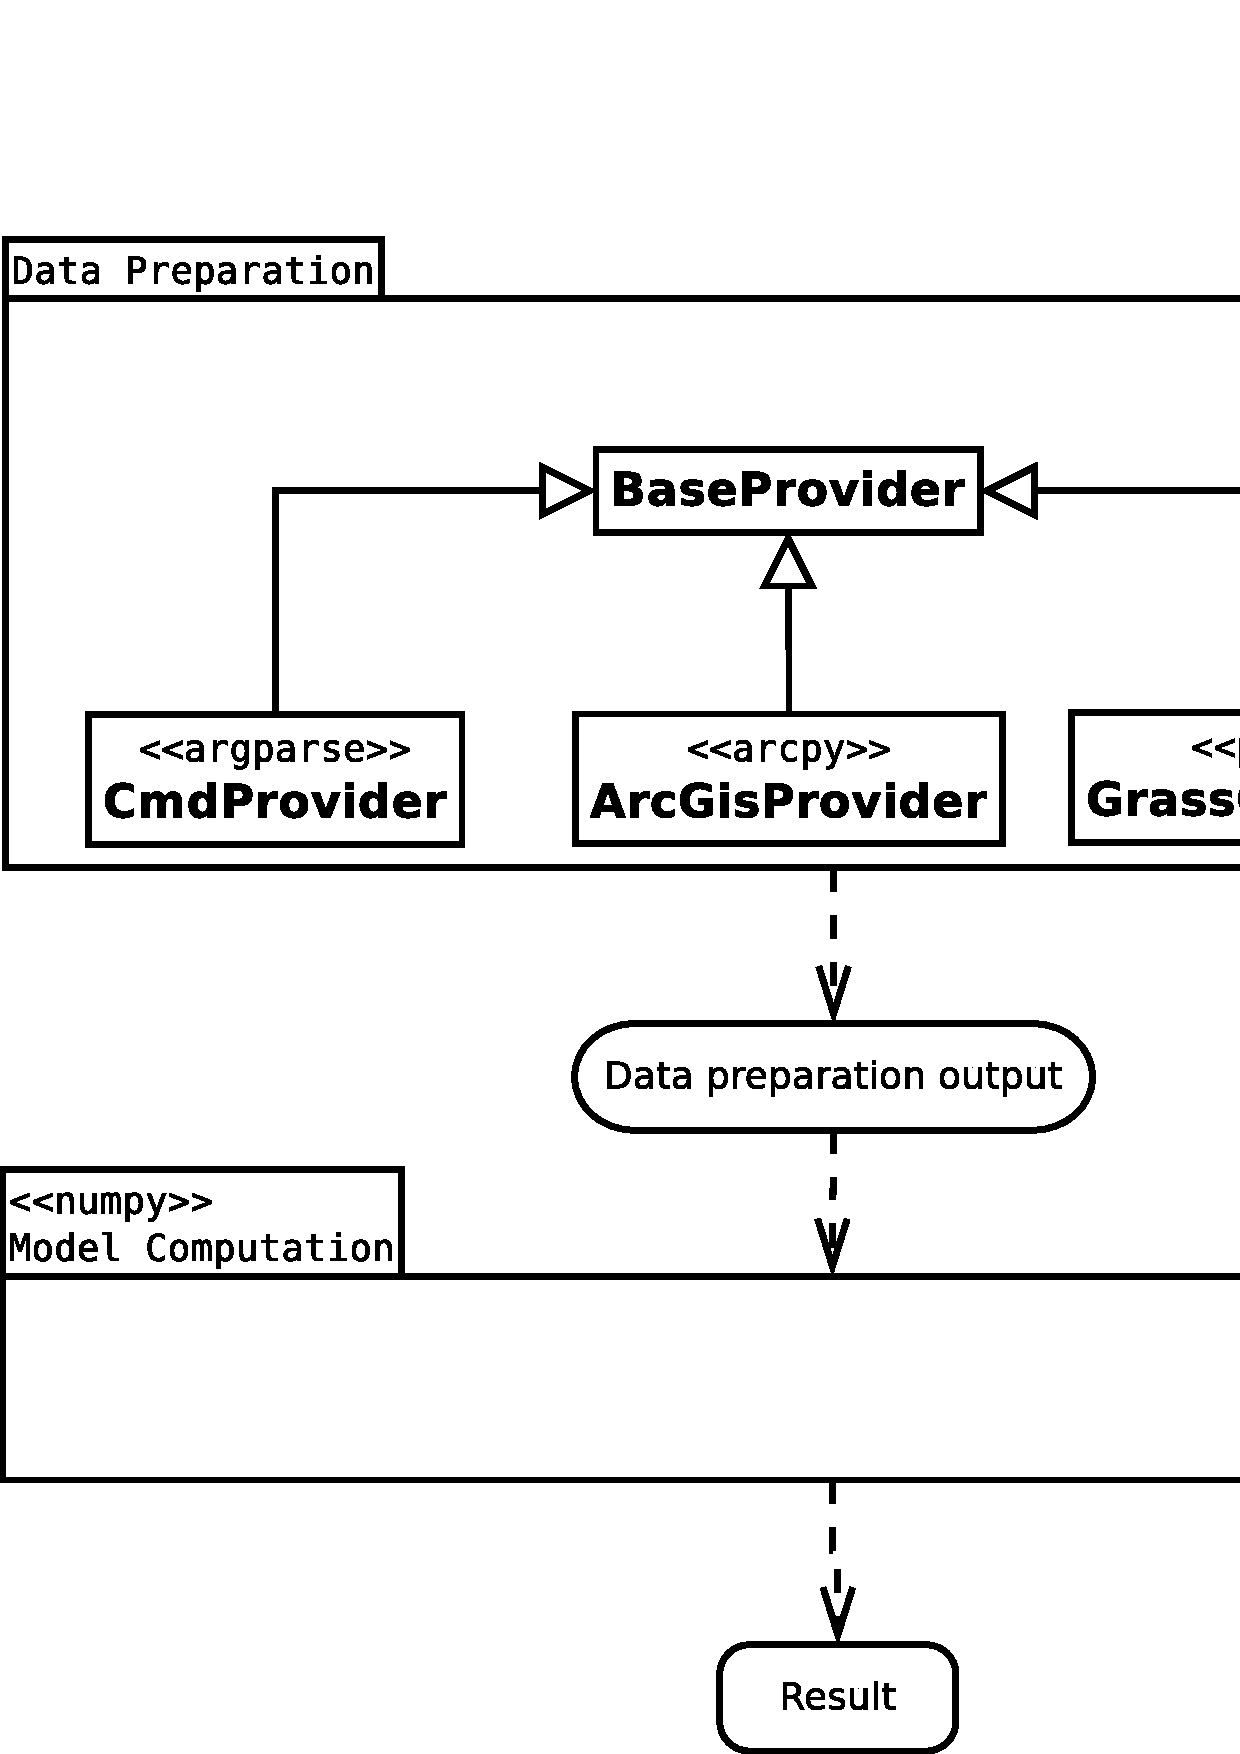
\includegraphics[width=1.0\columnwidth]{figures/uml_diagram.pdf}
    \caption{Data Preparation and Model Computation packages}
    \label{fig:uml_diagram}
  \end{center}
\end{figure}

\subsubsection{GRASS GIS implementation:}\label{sec:grass_provider}
Importantly, the new SMODER2D version extends supported GIS providers
by a GRASS-based provider. Introducing an open source GIS platform to
SMODERP2D workflow is crucial from the perspective of
interoperability. SMODERP2D users can choose between a proprietary
Esri ArcGIS platform and an open source GRASS
GIS\footnote{http://grass.osgeo.org}. The GRASS provider is designed
similarly to ArcGIS provider. From a Python perspective, there is only
one difference, GIS functions are accessed by PyGRASS package
\cite{ijgi2010201}. Integration of GRASS tools in SMODERP2D project
required few improvements on GRASS GIS side. That was possible since
GRASS GIS is an open source project available under GNU GPL
licence. GRASS v.to.points module \cite{v-to-points-2019} has been
extended to extract from lines start or end nodes only. This
functionality is used to determine the slope of a polyline stream
feature to ensure that its direction will always be downslope (see
fig. \ref{fig:stream_next_edge}). Another improvement has been done in
v.to.db GRASS module \cite{v-to-db-2019}. This tool allows uploading
geometry-related information into the attribute table. Newly added
option {\it next\_edge} allows adding information about next left and
right edge. This feature is important for SMODERP2D in order to
determine for each stream segment a previous segment.

\begin{figure}[ht!]
  \begin{center}
    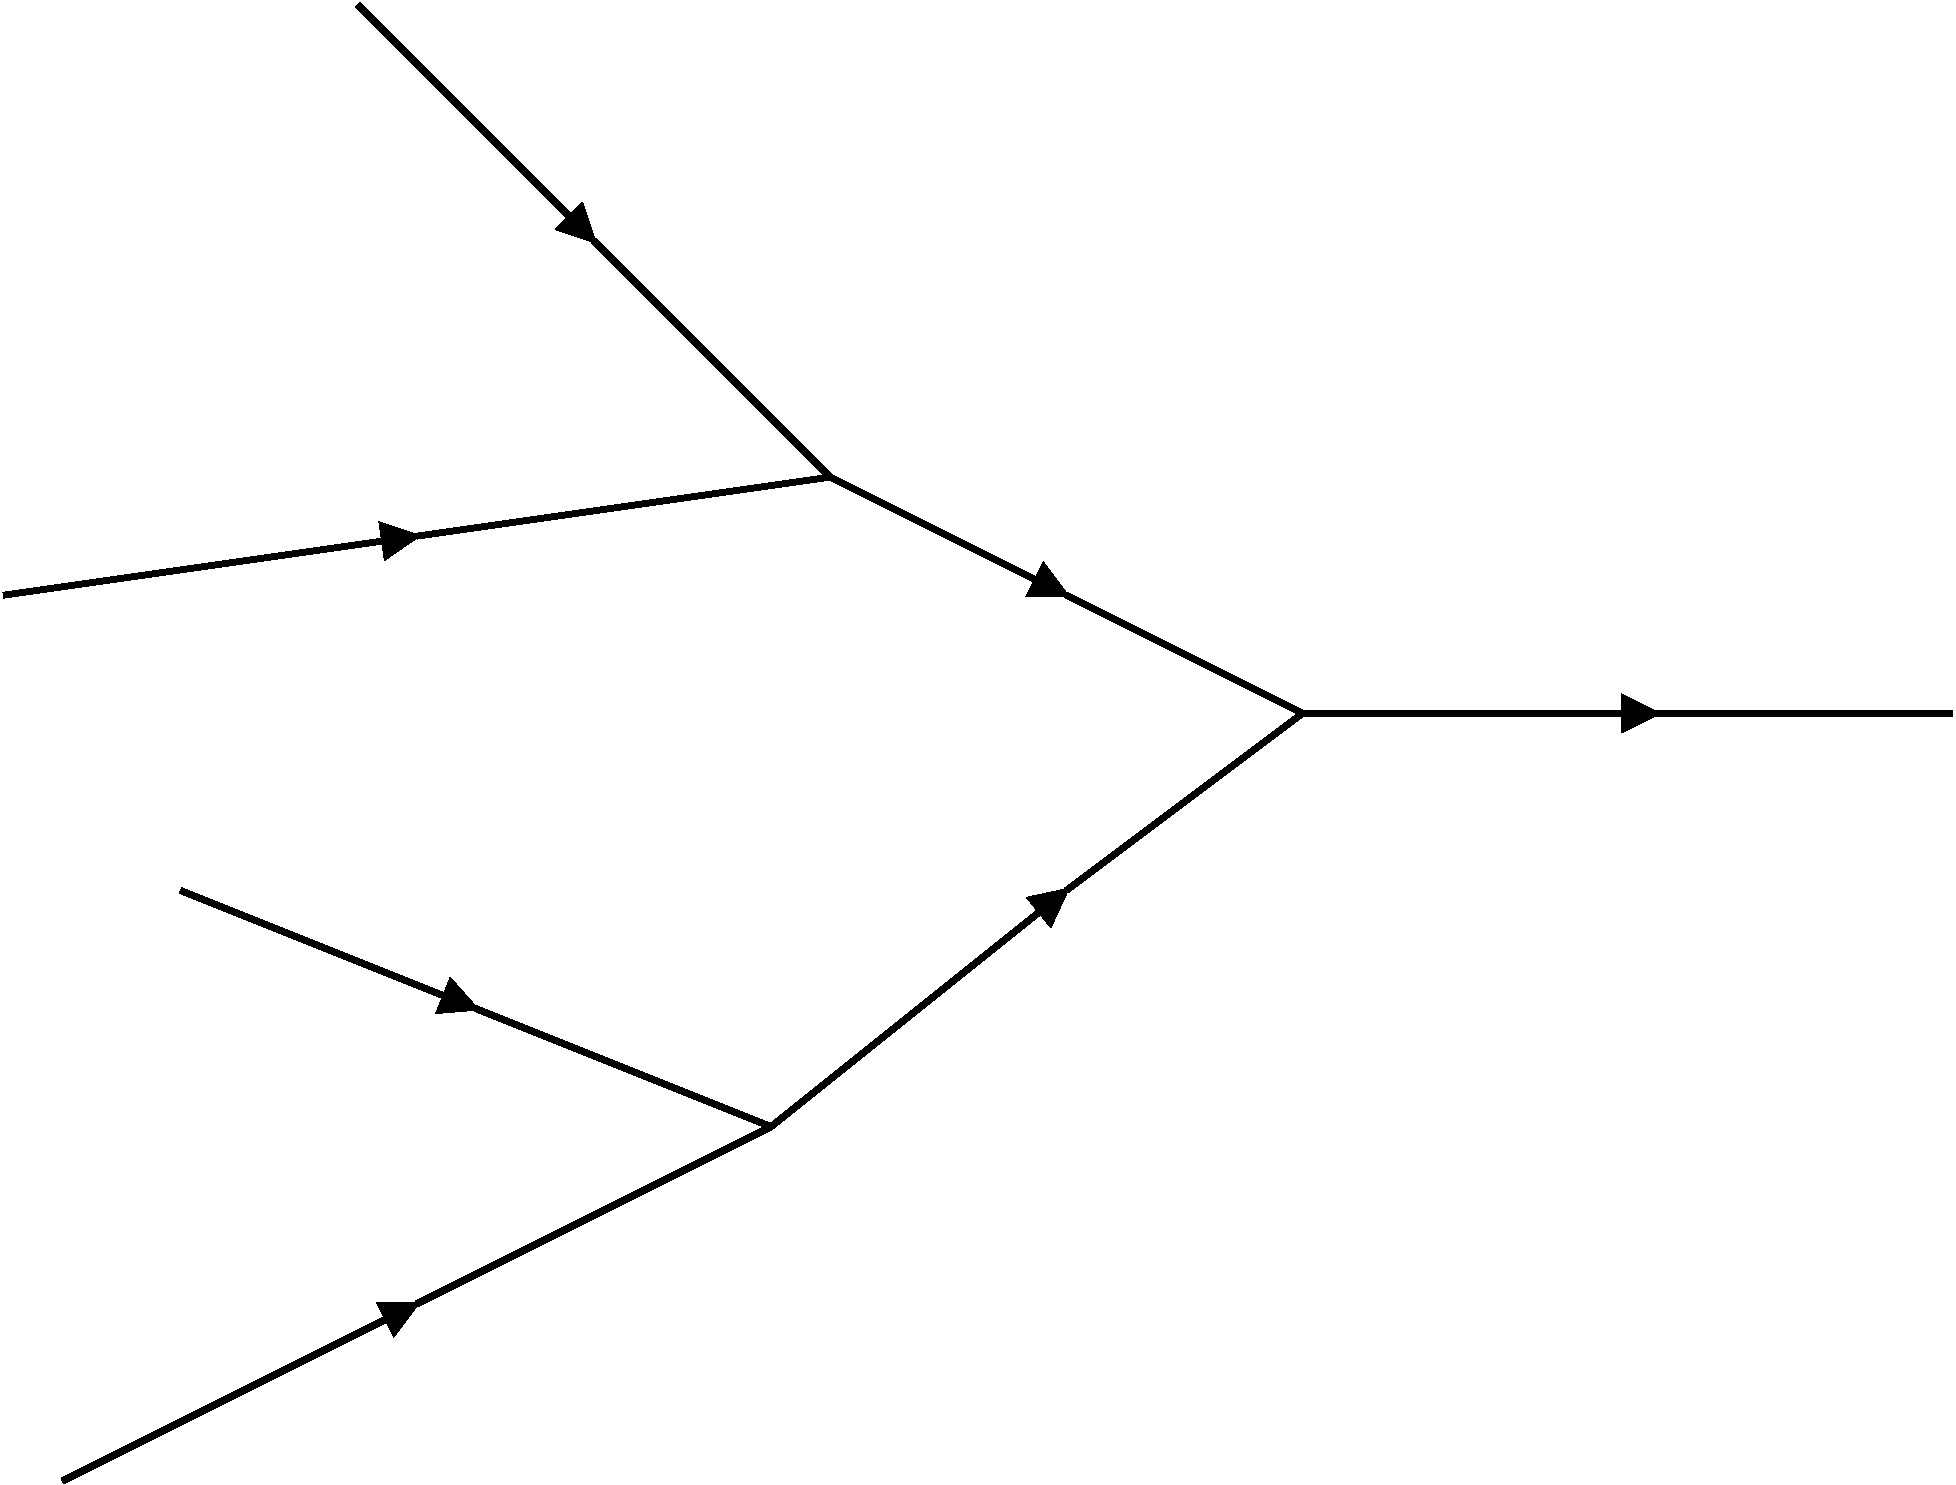
\includegraphics[width=0.6\columnwidth]{figures/stream_next_edge}
    \caption{Stream segmentation procedure: direction downslope}
    \label{fig:stream_next_edge}
  \end{center}
\end{figure}

On the top of GRASS GIS provider a specialized GRASS {\em r.smoderp2d}
module has been designed. This tool allows a user running SMODERP2D
model computation directly from GRASS GIS environment. The module can
be easily installed in GRASS GIS similarly to other extensions
(so-called addons modules) by {\em g.extension} command. By default,
the {\em r.smoderp2d} module performs data preparation phase followed by
model computation. Data preparation only can be performed by {\em -d}
flag. In this case, the module creates a binary pickle file which can
be later used for a subsequent model computation. Note that ArcGIS
Toolbox also allows creating a pickle file for later
usage. Importantly, such pickle files are platform independent.

Command-line usage example:
\begin{verbatim}
r.smoderp2d elevation=w001001 soil=soil_map \
 soil_type=Novak vegetation=soil_map \
 vegetation_type=veg rainfall_file=rainfall.txt \
 points=points2 table_soil_vegetation=tab_sv \
 table_soil_vegetation_code=soilveg \
 table_stream_shape=tab_stream_shape \
 table_stream_shape_code=smoderp stream=stream 
\end{verbatim}

\begin{figure}[ht!]
  \begin{center}
    \includegraphics[width=1.0\columnwidth]{figures/smoderp2d_grass.png}
    \caption{Running r.smoderp2d module from GRASS graphical user interface}
    \label{fig:uml_diagram}
  \end{center}
\end{figure}

\subsubsection{QGIS plugin:}
Recently the SMODERP2D model has been integrated also into QGIS
environment. QGIS\footnote{https://www.qgis.org} is a widely used open
source GIS platform which can be easily extended by user-defined
plugins. A SMODERP2D QGIS plugin (fig.~\ref{fig:smoderp2_qgis}) allows
performing both data preparatation and model computation parts (see
fig. \ref{fig:uml_diagram}) in QGIS native environment. Data
preparation part is ensured by GRASS GIS provider as described in
\ref{sec:grass_provider}. Note that QGIS installation normally comes
with GRASS GIS included. It means that GRASS dependency is solved by
QGIS installation itself. Experimental code of the plugin compatible
with current long term release QGIS version 3.4 is available from
project GitHub repository \cite{smoderp2d-github-2019}.

\begin{figure}[ht!]
  \begin{center}
    \includegraphics[width=1.0\columnwidth]{figures/smoderp2d_qgis.png}
    \caption{SMODERP2D model implemented as QGIS plugin}
    \label{fig:smoderp2_qgis}
  \end{center}
\end{figure}

\subsubsection{Python3 support:}
SMODERP2D in the new version also comes with Python 3 support, but
still supporting Python 2. Note that Python versions 2 and 3 are not
backward compatible.  Python 3 support is important from various
perspectives. Python 2 is slowly reaching end of life (ref), but still
it’s used by many GIS platforms such Esri ArcGIS 10.x. New generation
of SMODERP2D-supported GIS platforms like Esri ArcGIS Pro, (upcoming)
GRASS GIS 7.8 and QGIS 3.x are Python 3 based. On the other hand it’s
still meaningful to support both Python versions, Python 2 mainly
because of Esri ArcGIS 10.x platform.

\begin{figure}[ht!]
  \begin{center}
    \includegraphics[width=1.0\columnwidth]{figures/smoderp2d_arcgis.png}
    \caption{SMODERP2D model implemented as ArcToolbox for Esri ArcGIS
      10.x and Pro}
    \label{fig:uml_diagram}
  \end{center}
\end{figure}
